\documentclass{amsart}

\usepackage{amssymb}
\usepackage{booktabs}
\usepackage{tikz}
\usepackage[hidelinks]{hyperref}
\hypersetup{pdftitle={Domination polynomials with only real roots},pdfauthor={Knowledge Sense}}

\newtheorem{theorem}{Theorem}[section]
\newtheorem{lemma}[theorem]{Lemma}
\newtheorem{proposition}[theorem]{Proposition}
\newtheorem{corollary}[theorem]{Corollary}
\theoremstyle{definition}
\newtheorem{example}[theorem]{Example}
\theoremstyle{remark}
\newtheorem{remark}[theorem]{Remark}

\numberwithin{equation}{section}

\newcommand{\Z}{\mathbb{Z}}
\newcommand{\Q}{\mathbb{Q}}
\newcommand{\rhom}{\rho_-}
\newcommand{\rhop}{\rho_+}

\begin{document}

\title{Domination polynomials with only real roots}

\author{Knowledge Sense}
\address{Knowledge Sense}
\email{math@knowledgesense.jp}

\date{9 October 2026}

\subjclass[2020]{Primary 05C31; Secondary 05C69, 11R06}

\keywords{domination polynomial, domination root, real-rooted polynomial, dominating set, totally positive algebraic integer}

\begin{abstract}
The domination polynomial $D(H,x)$ of a finite simple graph $H$ counts the dominating sets of $H$ by size. We prove that all roots of $D(H,x)$ are real if and only if $H$ is obtained from a graph, possibly with no vertices, by attaching one or two pendant vertices to each of its vertices and then adding any number of isolated vertices. Oboudi proved that these graphs have only real domination roots and conjectured the converse. The proof combines the three leading coefficients of $D(H,x)$ with an inequality for monic integer polynomials whose roots are positive real numbers different from $1$: the sum of $\lambda^2-\lambda$ over the roots is at least twice the degree, with equality exactly for products of $z-2$ and $z^2-3z+1$. This inequality follows from a theorem of Liang and Wu; we also give a short self-contained proof. As a consequence, the domination roots of such a graph lie in $\{0,-2,(-3\pm\sqrt5)/2\}$, and we determine the connected graphs with exactly these four distinct domination roots.
\end{abstract}

\maketitle

\section{Introduction}

All graphs in this paper are finite and simple. For a graph $H$, a set $S\subseteq V(H)$ is \emph{dominating} if every vertex outside $S$ has a neighbour in $S$. Let $d_k(H)$ be the number of dominating sets of $H$ with $k$ elements. The \emph{domination polynomial}
\[
D(H,x)=\sum_{k\ge 0} d_k(H)\,x^k
\]
was introduced by Alikhani and Peng~\cite{AP14}, and its roots are called the \emph{domination roots} of $H$. We allow the graph $K_0$ with no vertices; since the empty set dominates it, $D(K_0,x)=1$. The smallest $k$ with $d_k(H)>0$ is the \emph{domination number} $\gamma(H)$.

Alikhani and his coauthors characterized several classes of graphs with few distinct domination roots; see the surveys~\cite{Ali11s,Ali13}. Brown and Tufts~\cite{BT14} showed that domination roots are dense in the complex plane, and Beaton and Brown~\cite{BB21} showed that the closure of the set of real domination roots is $(-\infty,0]$. Since the coefficients of $D(H,x)$ are nonnegative, real domination roots are nonpositive, and $-1$ is never a domination root~\cite{Obo16}.

For a graph $G$, possibly with no vertices, and a function $s\colon V(G)\to\{1,2,3,\dots\}$, let $G^s$ be the graph obtained from $G$ by adding, for every $v\in V(G)$, exactly $s(v)$ new vertices adjacent only to $v$. If $s\equiv 1$, then $G^s$ is the corona $G\circ K_1$. Oboudi~\cite[Theorem~3]{Obo16} computed $D(G^s,x)$ for every such $s$ (Lemma~\ref{lem:factor} below). In particular~\cite[Theorem~4]{Obo16}, if $s$ takes values in $\{1,2\}$, then
\begin{equation}\label{eq:formula}
D(G^s,x)=x^{a+b}(x+2)^a(x^2+3x+1)^b,\qquad a=|s^{-1}(1)|,\ b=|s^{-1}(2)|,
\end{equation}
so that $D(G^s,x)$ has only real roots. Adding $t$ isolated vertices multiplies the domination polynomial by $x^t$. Oboudi conjectured that the graphs $G^s\cup tK_1$ with $s$ taking values in $\{1,2\}$ are the only graphs whose domination polynomials have only real roots~\cite[Conjecture~1]{Obo16}. For graphs without isolated vertices, these are the \emph{star-like} graphs of Beaton and Cameron~\cite{BC24}, who mention the conjecture in their concluding discussion. In this paper we prove this conjecture.

\begin{theorem}\label{thm:main}
Let $H$ be a graph. Then all roots of $D(H,x)$ are real if and only if
\[
H\cong G^s\cup tK_1
\]
for some graph $G$, possibly with no vertices, some function $s\colon V(G)\to\{1,2\}$ and some integer $t\ge 0$. In this case
\[
D(H,x)=x^{a+b+t}(x+2)^a(x^2+3x+1)^b,\qquad a=|s^{-1}(1)|,\ b=|s^{-1}(2)|.
\]
\end{theorem}

The \emph{if} part and the formula are due to Oboudi; the new part is the converse. The graph $H$ need not be connected; isolated vertices, components $K_2$ (which are $K_1^s$ with $s\equiv1$) and the graph $K_0$ are included. Section~\ref{sec:consequences} proves the following consequences.

\begin{corollary}\label{cor:equiv}
For a graph $H$ the following are equivalent:
\begin{enumerate}
\item[(a)] all domination roots of $H$ are real;
\item[(b)] all domination roots of $H$ lie in $\{0,-2,(-3+\sqrt5)/2,(-3-\sqrt5)/2\}$;
\item[(c)] $H\cong G^s\cup tK_1$ with $G$, $s$ and $t$ as in Theorem~\ref{thm:main}.
\end{enumerate}
If they hold, then $\gamma(H)=a+b+t$ and $H$ has exactly $3^a5^b$ dominating sets.
\end{corollary}

\begin{corollary}\label{cor:four}
A connected graph $H$ has exactly the four distinct domination roots $0$, $-2$ and $(-3\pm\sqrt5)/2$ if and only if $H\cong G^s$ for a connected graph $G$ with at least one vertex and a function $s\colon V(G)\to\{1,2\}$ that takes both values.
\end{corollary}

\subsection*{The method}
Let $H$ be a graph with $n\ge 3$ vertices, $L$ leaves, no isolated vertices and no component $K_2$, and suppose that $D(H,x)$ has only real roots. By a theorem of Brouwer, every graph has an odd number of dominating sets, so $-1$ is not a root. Hence the negatives of the nonzero roots are the roots of a monic polynomial with integer coefficients whose roots are positive real numbers different from $1$; its degree is $n-\gamma(H)$. The three leading coefficients of $D(H,x)$ are $1$, $n$ and $\binom n2-L$, and this gives $\sum_i(\lambda_i^2-\lambda_i)=2L$ for these roots $\lambda_i$. The following lemma then yields $L\ge n-\gamma(H)$.

\begin{lemma}\label{lem:trace}
Let $p\in\Z[z]$ be a monic polynomial of degree $d\ge0$ whose roots $\lambda_1,\dots,\lambda_d$, listed with multiplicity, are positive real numbers different from $1$. Then
\[
\sum_{i=1}^d(\lambda_i^2-\lambda_i)\ \ge\ 2d,
\]
with equality if and only if $p=(z-2)^{\alpha}(z^2-3z+1)^{\beta}$ for some integers $\alpha,\beta\ge0$.
\end{lemma}

On the other hand, the set of non-leaves dominates $H$, so $\gamma(H)\le n-L$. Hence equality holds in both bounds, and the two equality cases determine the structure of $H$.

Lemma~\ref{lem:trace} is closely related to the trace problem for totally positive algebraic integers, and we do not claim it as new: in Section~\ref{sec:trace} we derive it from a theorem of Liang and Wu~\cite[Theorem~1.4]{LW11} on the mean of the squares of the conjugates. The proof of that theorem uses an auxiliary function involving $76$ polynomials, which are not listed in~\cite{LW11} but are available from the authors~\cite[Section~3.3]{LW11}. Appendix~\ref{app:trace} gives an independent proof of the weaker Lemma~\ref{lem:trace} with a single auxiliary function, in the spirit of~\cite{Smy84} and~\cite[Section~2]{LW11}, whose minimum is certified by five exact rational computations.

\subsection*{Organization}
Section~\ref{sec:prelim} contains the factorization for the graphs $G^s$, the parity theorem and the three leading coefficients. Section~\ref{sec:trace} proves Lemma~\ref{lem:trace} from the theorem of Liang and Wu, and Section~\ref{sec:proof} proves Theorem~\ref{thm:main}. Section~\ref{sec:consequences} proves the corollaries, compares Corollary~\ref{cor:four} with a statement in the surveys~\cite{Ali11s,Ali13}, and relates Theorem~\ref{thm:main} to the average order of dominating sets studied in~\cite{BC24}. With Appendix~\ref{app:trace}, the paper is self-contained.

\section{Preliminaries}\label{sec:prelim}

For a vertex $v$ of a graph $H$, let $N[v]$ be its closed neighbourhood, and for $S\subseteq V(H)$ let $N[S]=\bigcup_{v\in S}N[v]$; thus $S$ is dominating if and only if $N[S]=V(H)$. A \emph{leaf} is a vertex of degree one, and a \emph{support vertex} is a vertex adjacent to a leaf. A set dominates a disjoint union $H_1\cup H_2$ if and only if its intersections with $V(H_1)$ and $V(H_2)$ dominate $H_1$ and $H_2$, so
\begin{equation}\label{eq:mult}
D(H_1\cup H_2,x)=D(H_1,x)\,D(H_2,x).
\end{equation}
In particular $D(K_1,x)=x$ and $D(K_2,x)=x^2+2x$.

The following product formula is~\cite[Theorem~3]{Obo16}; we include the short proof for completeness.

\begin{lemma}\label{lem:factor}
Let $G$ be a graph and $s\colon V(G)\to\{1,2,3,\dots\}$. Then
\[
D(G^s,x)=\prod_{v\in V(G)}\bigl(x(1+x)^{s(v)}+x^{s(v)}\bigr).
\]
In particular, $D(G^s,x)$ does not depend on the edges of $G$, and~\eqref{eq:formula} holds if $s$ takes values in $\{1,2\}$.
\end{lemma}

\begin{proof}
For $v\in V(G)$ let $A_v$ be the set of the $s(v)$ vertices attached to $v$. We claim that $S\subseteq V(G^s)$ is dominating if and only if, for every $v\in V(G)$, either $v\in S$ or $A_v\subseteq S$. Indeed, a vertex $u\in A_v$ has $N[u]=\{u,v\}$, so the condition is necessary. Conversely, if it holds, every $u\in A_v$ lies in $S$ or is adjacent to $v\in S$, and $v$ lies in $S$ or is adjacent to a vertex of the nonempty set $A_v\subseteq S$. The condition involves each block $\{v\}\cup A_v$ separately, and these blocks partition $V(G^s)$. The sets $S\cap(\{v\}\cup A_v)$ with $v\in S$ contribute $x(1+x)^{s(v)}$, and the only admissible set with $v\notin S$ is $A_v$, which contributes $x^{s(v)}$. This proves the product formula. For $s(v)=1$ and $s(v)=2$ the factors are $x(x+2)$ and $x(x^2+3x+1)$.
\end{proof}

Every graph has an odd number of dominating sets. This is due to Brouwer; see~\cite{Bro09}, which gives three proofs, by Brouwer, Csorba and Schrijver, and also~\cite[Theorem~5]{Obo16}. We include Schrijver's proof, phrased in terms of a bipartite graph.

\begin{lemma}\label{lem:parity}
For every graph $H$, the number $D(H,1)$ is odd. Consequently, $D(H,-1)$ is also odd, and $-1$ is not a domination root of $H$.
\end{lemma}

\begin{proof}
Let $V=V(H)$ and $n=|V|$. Consider the bipartite graph $B$ with two copies $V\times\{1\}$ and $V\times\{2\}$ of $V$, in which $(u,1)$ is adjacent to $(w,2)$ if and only if $w\in N[u]$. An independent set of $B$ is a pair of sets $A,C\subseteq V$, placed in the first and the second copy, with $C\cap N[A]=\emptyset$. For fixed $A$ there are $2^{\,n-|N[A]|}$ choices of $C$, so the number of independent sets of $B$ is
\[
\sum_{A\subseteq V}2^{\,n-|N[A]|}\equiv\bigl|\{A\subseteq V:\ N[A]=V\}\bigr|=D(H,1)\pmod 2.
\]
Since $w\in N[u]$ if and only if $u\in N[w]$, the map $(A,C)\mapsto(C,A)$ is an involution on the independent sets of $B$. A fixed point has $A=C$ and $A\cap N[A]=\emptyset$, hence $A=\emptyset$. The independent sets other than $(\emptyset,\emptyset)$ thus come in pairs, so their total number is odd. Finally $D(H,-1)\equiv D(H,1)\pmod 2$ because $D(H,x)$ has integer coefficients.
\end{proof}

\begin{lemma}\label{lem:top}
Let $H$ be a graph with $n\ge 3$ vertices, no isolated vertices and no component isomorphic to $K_2$, and let $L$ be the number of leaves of $H$. Then
\[
d_n(H)=1,\qquad d_{n-1}(H)=n,\qquad d_{n-2}(H)=\binom n2-L.
\]
\end{lemma}

\begin{proof}
A set $S$ fails to dominate $H$ if and only if $N[w]\subseteq V(H)\setminus S$ for some vertex $w$. Every closed neighbourhood has at least two elements, so every set with at least $n-1$ elements dominates. If $V(H)\setminus S=\{u,v\}$ with $u\neq v$, then $S$ fails to dominate if and only if $\{u,v\}=N[w]$ for some $w$, that is, $w\in\{u,v\}$ is a leaf whose neighbour is the other element of $\{u,v\}$. If two distinct leaves $w,w'$ had $N[w]=N[w']$, then $N[w]=\{w,w'\}$, and $w,w'$ would form a component $K_2$. Hence $w\mapsto N[w]$ is a bijection from the leaves onto the $2$-sets whose complements do not dominate, and $d_{n-2}(H)=\binom n2-L$.
\end{proof}

\section{The trace inequality}\label{sec:trace}

In this section we derive Lemma~\ref{lem:trace} from the work of Liang and Wu. For an algebraic integer $\lambda$ of degree $d$ with conjugates $\lambda_1,\dots,\lambda_d$ put $S_k=\sum_{i=1}^d\lambda_i^k$; recall that $\lambda$ is \emph{totally positive} if all $\lambda_i$ are positive real numbers. Liang and Wu proved~\cite[Theorem~1.4]{LW11} that every totally positive algebraic integer of degree $d\ge2$ satisfies
\begin{equation}\label{eq:LW}
\frac{S_2}{d}>5.31935
\end{equation}
unless its minimal polynomial is one of the following five polynomials, denoted $P_1,\dots,P_5$ in~\cite{LW11}:
\begin{align*}
E_1&=z^2-3z+1,\\
E_2&=z^3-5z^2+6z-1,\\
E_3&=z^5-9z^4+28z^3-35z^2+15z-1,\\
E_4&=z^6-11z^5+45z^4-84z^3+70z^2-21z+1,\\
E_5&=z^4-7z^3+14z^2-8z+1.
\end{align*}

\begin{proof}[Proof of Lemma~\ref{lem:trace}]
By Gauss's lemma, $p$ is a product of monic irreducible polynomials in $\Z[z]$, each of which again has positive real roots different from $1$. Both sides of the inequality are additive over such a factorization, so it suffices to show that every monic irreducible $p\in\Z[z]$ of degree $d\ge1$ with this property satisfies $S_2-S_1\ge 2d$, with equality if and only if $p\in\{z-2,\ z^2-3z+1\}$, where $S_k$ is the $k$-th power sum of the roots of $p$.

If $d=1$, then $p=z-k$ for an integer $k\ge2$, and $k^2-k\ge2$ with equality if and only if $k=2$. Let $d\ge2$. Then the roots of $p$ are the conjugates of a totally positive algebraic integer of degree $d$ with minimal polynomial $p$. Suppose first that $p\notin\{E_1,\dots,E_5\}$, and put $y=S_2/d$. By the Cauchy--Schwarz inequality, $S_1/d\le\sqrt{y}$, so
\[
\frac{S_2-S_1}{d}\ \ge\ y-\sqrt y\ >\ 5-\sqrt5\ >\ 2,
\]
because $y\mapsto y-\sqrt y$ is increasing for $y\ge 1/4$ and $y>5$ by~\eqref{eq:LW}. For the five exceptions, $S_1$ is minus the coefficient of $z^{d-1}$ and $S_2=S_1^2-2e_2$, where $e_2$ is the coefficient of $z^{d-2}$. This gives the following values of $(S_2-S_1)/d$:
\begin{gather*}
E_1\colon\ \tfrac{7-3}{2}=2,\qquad E_2\colon\ \tfrac{13-5}{3}=\tfrac83,\qquad E_3\colon\ \tfrac{25-9}{5}=\tfrac{16}5,\\
E_4\colon\ \tfrac{31-11}{6}=\tfrac{10}3,\qquad E_5\colon\ \tfrac{21-7}{4}=\tfrac72.
\end{gather*}
Thus $S_2-S_1\ge2d$, with equality only for $E_1$.
\end{proof}

\begin{remark}\label{rem:selfcontained}
Lemma~\ref{lem:trace} is sharp, by $z-2$ and $z^2-3z+1$, but much weaker than~\eqref{eq:LW}. Appendix~\ref{app:trace} proves it directly by showing that
\[
z^2-z-\log|z(z-1)^2(z-2)(z^2-3z+1)|>2
\]
for all $z>0$ at which the left-hand side is defined; Lemma~\ref{lem:trace} then follows by summing over the roots of $p$ and using that a nonzero resultant is an integer.
\end{remark}

\section{Proof of Theorem~\ref{thm:main}}\label{sec:proof}

\begin{proof}[Proof of Theorem~\ref{thm:main}]
If $H\cong G^s\cup tK_1$ with $s$ taking values in $\{1,2\}$, then~\eqref{eq:mult} and Lemma~\ref{lem:factor} give the stated formula, and all roots are real because $x^2+3x+1$ has the real roots $(-3\pm\sqrt5)/2$.

Conversely, suppose that all roots of $D(H,x)$ are real. Let $t$ be the number of isolated vertices of $H$, let $c$ be the number of components isomorphic to $K_2$, and let $H_0$ be the graph obtained from $H$ by deleting these vertices and components. By~\eqref{eq:mult},
\[
D(H,x)=x^t(x^2+2x)^c\,D(H_0,x),
\]
so $D(H_0,x)$ has only real roots. It suffices to show that $H_0\cong G_0^{s_0}$ for some graph $G_0$ and some $s_0\colon V(G_0)\to\{1,2\}$: then $H\cong G^s\cup tK_1$, where $G=G_0\cup cK_1$ and $s$ extends $s_0$ by the value $1$ on the $c$ new vertices. If $H_0$ has no vertices, we take $G_0=K_0$. Otherwise every component of $H_0$ has at least three vertices. Let $n\ge 3$ be the number of vertices of $H_0$, $L$ the number of its leaves and $\gamma=\gamma(H_0)$. We write $d_k=d_k(H_0)$.

\emph{Step 1: the roots.} By Lemma~\ref{lem:top}, $d_n=1$; since all coefficients are nonnegative, $D(H_0,x)>0$ for $x>0$, and the real roots of $D(H_0,x)$ are nonpositive. The root $0$ has multiplicity exactly $\gamma$, since $d_\gamma>0$, and $-1$ is not a root by Lemma~\ref{lem:parity}. Hence
\[
D(H_0,x)=x^\gamma\,g(x),\qquad g(x)=\prod_{i=1}^m(x+\lambda_i),\qquad m=n-\gamma,
\]
where $\lambda_1,\dots,\lambda_m$ are positive real numbers different from $1$. The polynomial $g$ is monic with integer coefficients $d_\gamma,\dots,d_n$, so $p(z)=(-1)^mg(-z)=\prod_{i=1}^m(z-\lambda_i)$ is a monic polynomial in $\Z[z]$.

\emph{Step 2: the trace.} Let $e_1$ and $e_2$ be the first two elementary symmetric functions of $\lambda_1,\dots,\lambda_m$, with $e_2=0$ if $m=1$. They are the coefficients of $x^{m-1}$ and $x^{m-2}$ in $g$, that is, $e_1=d_{n-1}$ and $e_2=d_{n-2}$. By Lemma~\ref{lem:top},
\[
\sum_{i=1}^m\lambda_i=n,\qquad \sum_{i=1}^m\lambda_i^2=e_1^2-2e_2=n^2-n(n-1)+2L=n+2L,
\]
and therefore
\begin{equation}\label{eq:2L}
\sum_{i=1}^m(\lambda_i^2-\lambda_i)=2L.
\end{equation}
Lemma~\ref{lem:trace}, applied to $p$, gives $2L\ge 2m$, that is, $\gamma\ge n-L$.

\emph{Step 3: the non-leaves.} The neighbour of a leaf of $H_0$ is not a leaf, since $H_0$ has no component $K_2$. Hence the set of non-leaves of $H_0$ dominates $H_0$, and $\gamma\le n-L$. Together with Step~2 we obtain
\begin{equation}\label{eq:equality}
\gamma=n-L,\qquad m=L,
\end{equation}
and equality holds in Lemma~\ref{lem:trace} for $p$. Consequently $p=(z-2)^\alpha(z^2-3z+1)^\beta$ for some $\alpha,\beta\ge0$, that is,
\begin{equation}\label{eq:H0}
D(H_0,x)=x^\gamma(x+2)^\alpha(x^2+3x+1)^\beta.
\end{equation}

\emph{Step 4: every non-leaf is a support vertex.} Suppose that a non-leaf $v$ of $H_0$ has no leaf neighbour, and let $S$ be the set of non-leaves other than $v$. Every leaf is adjacent to a non-leaf different from $v$, which lies in $S$. The vertex $v$ has a neighbour, as $H_0$ has no isolated vertices, and all neighbours of $v$ are non-leaves different from $v$, hence lie in $S$. Thus $S$ dominates $H_0$ and $|S|=n-L-1<\gamma$, contradicting~\eqref{eq:equality}.

\emph{Step 5: one or two leaves at each support vertex.} Let $G_0$ be the subgraph of $H_0$ induced by the non-leaves, and for $v\in V(G_0)$ let $s_0(v)\ge1$ be the number of leaves adjacent to $v$. By Steps~3 and~4, every leaf is adjacent to exactly one vertex of $G_0$, so $H_0=G_0^{s_0}$. Let $v\in V(G_0)$ with $s=s_0(v)\ge2$. By Lemma~\ref{lem:factor}, the polynomial
\[
f_s(x)=(1+x)^s+x^{s-1}
\]
divides $D(H_0,x)$. Since $f_s$ is monic with $f_s(0)=1$, and $x+2$ and $x^2+3x+1$ are irreducible over $\Q$, unique factorization in $\Q[x]$ and~\eqref{eq:H0} give
\[
f_s(x)=(x+2)^{\alpha'}(x^2+3x+1)^{\beta'},\qquad \alpha',\beta'\ge0.
\] Comparing constant terms gives $2^{\alpha'}=1$, so $\alpha'=0$. Comparing degrees gives $s=2\beta'$, and comparing the coefficients of $x^{s-1}$ gives $s+1=3\beta'$. Hence $\beta'=1$ and $s=2$. Therefore $s_0$ takes values in $\{1,2\}$, which completes the proof.
\end{proof}

\section{Consequences}\label{sec:consequences}

\subsection{The corollaries}

\begin{proof}[Proof of Corollary~\ref{cor:equiv}]
The implication (c)$\Rightarrow$(b) follows from the formula in Theorem~\ref{thm:main}, (b)$\Rightarrow$(a) is trivial, and (a)$\Rightarrow$(c) is Theorem~\ref{thm:main}. Under (c), the lowest power of $x$ in $D(H,x)$ is $x^{a+b+t}$, with coefficient $2^a$, so $\gamma(H)=a+b+t$, and $D(H,1)=3^a5^b$.
\end{proof}

\begin{proof}[Proof of Corollary~\ref{cor:four}]
If $H\cong G^s$ with $G$ and $s$ as stated, then $H$ is connected and, by Theorem~\ref{thm:main}, its distinct domination roots are $0$, $-2$ and $(-3\pm\sqrt5)/2$, because $a\ge1$ and $b\ge1$. Conversely, if a connected graph $H$ has these four distinct domination roots, then all its domination roots are real, and $H\cong G^s\cup tK_1$ by Theorem~\ref{thm:main}. Since $H$ has a nonzero domination root, $H\neq K_1$; as $H$ is connected, $t=0$ and $G$ is connected with at least one vertex. The roots $-2$ and $(-3\pm\sqrt5)/2$ occur only if $a\ge1$ and $b\ge1$.
\end{proof}

Theorem~\ref{thm:main} gives a simple test: $D(H,x)$ has only real roots if and only if, after the deletion of the isolated vertices of $H$ and of its components isomorphic to $K_2$, every vertex that is not a leaf is adjacent to one or two leaves. In particular, real-rootedness of $D(H,x)$ can be decided in linear time.

The case $b=0$ of Theorem~\ref{thm:main} concerns the graphs all of whose domination roots are integers; these were determined by Oboudi~\cite[Theorem~13]{Obo16}. Similarly, Theorem~\ref{thm:main} shows that the connected graphs whose sets of distinct domination roots are $\{0,-2\}$ and $\{0,(-3\pm\sqrt5)/2\}$ are the coronas $G\circ K_1$ and the graphs $G^s$ with $s\equiv2$, respectively, with $G$ connected; these characterizations are stated in~\cite[Theorems~5 and~6]{Ali11s}.

Akbari, Alikhani, Oboudi and Peng~\cite{AAOP10} conjectured that every integer domination root lies in $\{0,-2\}$, and Alikhani and Griswold~\cite{AG26} recently found a graph with the domination root $-4$. By Corollary~\ref{cor:equiv}, the conjecture holds for graphs whose domination polynomials have only real roots, so every graph with an integer domination root outside $\{0,-2\}$, such as this one, also has non-real domination roots.

\subsection{Connected graphs with four distinct domination roots}

The surveys~\cite[Theorem~10]{Ali11s} and~\cite[Theorem~12, Eq.~(4)]{Ali13} state that a connected graph $G$ of order $n$ has the distinct domination roots $0$, $-2$ and $(-3\pm\sqrt5)/2$ if and only if $G$ is obtained from a corona $G_{n/2}\circ K_1$ of a graph $G_{n/2}$ of order $n/2$ by deleting one vertex, and that then
\begin{equation}\label{eq:survey}
D(G,x)=(x^2+3x+1)\,x^{n/2-1}(x+2)^{n/2-2}.
\end{equation}
Deleting a vertex from the corona of a graph with $k$ vertices leaves $2k-1$ vertices, and the polynomial in~\eqref{eq:survey} has degree $n-1$ rather than $n$, so the indices do not match. Under any reading of the indices, however, the polynomial~\eqref{eq:survey} contains the factor $x^2+3x+1$ exactly once, so the following graph is not covered by the statement in the surveys.

\begin{example}\label{ex:tree}
Let $T$ be the tree with vertex set $\{0,1,\dots,7\}$ and edges
\[
01,\ 12,\ 03,\ 04,\ 15,\ 26,\ 27;
\]
see Figure~\ref{fig:tree}. Then $T=P_3^s$ for the path $P_3$ on $0,1,2$ and $s(0)=2$, $s(1)=1$, $s(2)=2$. By Lemma~\ref{lem:factor},
\[
D(T,x)=x^3(x+2)(x^2+3x+1)^2=x^8+8x^7+23x^6+28x^5+13x^4+2x^3,
\]
as can also be checked by enumerating the $256$ subsets of $V(T)$. Thus $T$ is a connected graph whose distinct domination roots are exactly $0$, $-2$ and $(-3\pm\sqrt5)/2$. It has an even number of vertices, and $(x^2+3x+1)^2$ divides $D(T,x)$.
\end{example}

\begin{figure}[ht]
\centering
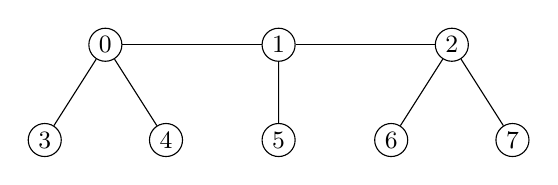
\begin{tikzpicture}[every node/.style={circle,draw,fill=white,inner sep=1.6pt,font=\small},scale=1.1]
\node (v0) at (0,0) {$0$};
\node (v1) at (2,0) {$1$};
\node (v2) at (4,0) {$2$};
\node (v3) at (-0.7,-1.1) {$3$};
\node (v4) at (0.7,-1.1) {$4$};
\node (v5) at (2,-1.1) {$5$};
\node (v6) at (3.3,-1.1) {$6$};
\node (v7) at (4.7,-1.1) {$7$};
\draw (v0)--(v1)--(v2);
\draw (v0)--(v3); \draw (v0)--(v4); \draw (v1)--(v5); \draw (v2)--(v6); \draw (v2)--(v7);
\end{tikzpicture}
\caption{The tree $T$ of Example~\ref{ex:tree}.}
\label{fig:tree}
\end{figure}

By Corollary~\ref{cor:four}, the connected graphs with these four distinct domination roots are exactly the graphs $G^s$ with $G$ connected and $s$ taking both values $1$ and $2$; their domination polynomials are $x^{a+b}(x+2)^a(x^2+3x+1)^b$ with $a,b\ge1$, and their orders $2a+3b$ are the integers $n\ge5$ with $n\ne6$. If the order in~\cite[Theorem~10]{Ali11s} is read as $2k-1$, then~\eqref{eq:survey} becomes $(x^2+3x+1)x^{k-1}(x+2)^{k-2}$, which is the domination polynomial of the graphs in Corollary~\ref{cor:four} with $b=1$.

\subsection{The average order of dominating sets}

For a graph $H$ with $n$ vertices, the average order of a dominating set is $\operatorname{avd}(H)=D'(H,1)/D(H,1)$. Beaton and Cameron~\cite[Theorem~2.10]{BC24} proved that $\operatorname{avd}(H)\le 2n/3$ for every graph $H$ with $n\ge2$ vertices and no isolated vertices, with equality if and only if $H$ is star-like, that is, $H\cong G^s$ with $s$ taking values in $\{1,2\}$; they also deduced the bound $\operatorname{avd}(H)\le(2n+t)/3$ for graphs with $t$ isolated vertices~\cite[Corollary~2.11]{BC24}. Since $\operatorname{avd}$ is additive over disjoint unions by~\eqref{eq:mult} and $\operatorname{avd}(tK_1)=t$, their equality case extends to graphs with isolated vertices. Combined with Theorem~\ref{thm:main}, this gives the following equivalence.

\begin{corollary}\label{cor:avd}
Let $H$ be a graph with $n$ vertices, $t$ of which are isolated. Then all domination roots of $H$ are real if and only if $\operatorname{avd}(H)=(2n+t)/3$.
\end{corollary}

For the graphs in Theorem~\ref{thm:main} the value can also be computed directly: the logarithmic derivative of $x^{a+b+t}(x+2)^a(x^2+3x+1)^b$ at $x=1$ is $a+b+t+a/3+b=(2n+t)/3$, because $n=2a+3b+t$.

\appendix

\section{A self-contained proof of Lemma~\ref{lem:trace}}\label{app:trace}

Put
\[
Q(z)=z(z-1)^2(z-2)(z^2-3z+1),\qquad F(z)=z^2-z-\log|Q(z)|,
\]
and let $\rhom=(3-\sqrt5)/2$ and $\rhop=(3+\sqrt5)/2$ be the roots of $z^2-3z+1$.

\begin{proposition}\label{prop:aux}
For every real $z>0$ with $Q(z)\neq0$, we have $F(z)>2$.
\end{proposition}

\begin{proof}
The positive zeros of $Q$ divide $(0,\infty)$ into the five open intervals
\[
I_1=(0,\rhom),\quad I_2=(\rhom,1),\quad I_3=(1,2),\quad I_4=(2,\rhop),\quad I_5=(\rhop,\infty).
\]
On each $I_j$ the function $F$ is smooth, with
\begin{align}
F'(z)&=2z-1-\frac1z-\frac{2}{z-1}-\frac{1}{z-2}-\frac{2z-3}{z^2-3z+1},\label{eq:Fprime}\\
F''(z)&=2+\frac1{z^2}+\frac2{(z-1)^2}+\frac1{(z-2)^2}+\frac1{(z-\rhom)^2}+\frac1{(z-\rhop)^2}>0.\notag
\end{align}
Thus $F'$ is strictly increasing on $I_j$. Table~\ref{tab:cert} lists rational numbers $\sigma_j<\tau_j$ with $[\sigma_j,\tau_j]\subset I_j$. Evaluating~\eqref{eq:Fprime} exactly in rational arithmetic gives $F'(\sigma_j)<0<F'(\tau_j)$ for $j=1,\dots,5$. Hence $F'$ has a unique zero $c_j\in(\sigma_j,\tau_j)$, and $F(c_j)$ is the minimum of $F$ on $I_j$. It therefore suffices to show $F>2$ on $[\sigma_j,\tau_j]$.

Fix $j$, write $[\sigma,\tau]=[\sigma_j,\tau_j]$, and define the rational numbers
\begin{align*}
u&=\min_{\sigma\le z\le \tau}(z^2-z-2),\\
R&=\tau\cdot\max\{|\sigma-1|,|\tau-1|\}^2\cdot\max\{|\sigma-2|,|\tau-2|\}\cdot\max_{\sigma\le z\le \tau}|z^2-3z+1|.
\end{align*}
The extrema of the quadratic polynomials occur at $\sigma$, at $\tau$, or at their vertices $1/2$ and $3/2$ if these lie in $[\sigma,\tau]$, so $u$ and $R$ are rational, and $|Q(z)|\le R$ for $z\in[\sigma,\tau]$. By Taylor's theorem with the Lagrange remainder, which is a nonnegative multiple of $u^{20}$, we have
\[
e^u\ \ge\ T_{19}(u)=\sum_{k=0}^{19}\frac{u^k}{k!}.
\]
Table~\ref{tab:cert} gives $u$ and integers $\ell$ and $r$ with $\ell\le10^6\,T_{19}(u)$ and $10^6R\le r$; in every row $\ell>r$. Hence, for $z\in[\sigma,\tau]$,
\[
|Q(z)|\le R\le\frac{r}{10^6}<\frac{\ell}{10^6}\le T_{19}(u)\le e^u\le e^{z^2-z-2},
\]
that is, $F(z)>2$.
\end{proof}

\begin{table}[ht]
\centering
\caption{Certificates for Proposition~\ref{prop:aux}. Here $\ell=\lfloor 10^6\,T_{19}(u)\rfloor$ and $r=\lceil 10^6R\rceil$.}
\label{tab:cert}
\begin{tabular}{@{}cccccrr@{}}
\toprule
$j$ & $I_j$ & $\sigma_j$ & $\tau_j$ & $u$ & $\ell$ & $r$\\
\midrule
$1$ & $(0,\rhom)$ & $0.1464$ & $0.1465$ & $-8500151/4000000$ & $119428$ & $115202$\\
$2$ & $(\rhom,1)$ & $0.5960$ & $0.5961$ & $-140049/62500$ & $106375$ & $59143$\\
$3$ & $(1,2)$ & $1.5422$ & $1.5423$ & $-29095479/25000000$ & $312291$ & $259188$\\
$4$ & $(2,\rhop)$ & $2.2636$ & $2.2637$ & $5376781/6250000$ & $2363834$ & $635752$\\
$5$ & $(\rhop,\infty)$ & $3.0332$ & $3.0333$ & $26044389/6250000$ & $64528192$ & $14267095$\\
\bottomrule
\end{tabular}
\end{table}

All entries of Table~\ref{tab:cert} were computed in exact rational arithmetic. Numerically, the minima are $F(c_j)\approx 2.037$, $2.588$, $2.187$, $3.314$ and $3.510$.

\begin{proof}[Second proof of Lemma~\ref{lem:trace}]
As in Section~\ref{sec:trace}, it suffices to treat a monic irreducible $p\in\Z[z]$ of degree $d\ge1$ whose roots $\lambda_1,\dots,\lambda_d$ are positive and different from $1$. If $p$ has a root in common with $Q$, then $p$ divides $Q$, because $p$ is irreducible over $\Q$. The monic irreducible factors of $Q$ are $z$, $z-1$, $z-2$ and $z^2-3z+1$; the first two are excluded by the hypotheses, and for the other two $\sum_i(\lambda_i^2-\lambda_i)$ equals $2$ and $7-3=4$, respectively, so equality holds. Otherwise $Q(\lambda_i)\neq0$ for all $i$, and $\prod_iQ(\lambda_i)$ is the resultant of $p$ and $Q$, a nonzero integer. Hence $\sum_i\log|Q(\lambda_i)|\ge0$, and Proposition~\ref{prop:aux} gives
\[
\sum_{i=1}^d(\lambda_i^2-\lambda_i)\ >\ 2d+\sum_{i=1}^d\log|Q(\lambda_i)|\ \ge\ 2d.
\]
Summing over the irreducible factors proves the inequality, and equality holds exactly when every factor is $z-2$ or $z^2-3z+1$.
\end{proof}

\section*{Use of AI-assisted tools}

AI-assisted tools were used in the research and preparation of this manuscript.

\begin{thebibliography}{99}

\bibitem{AAOP10}
S. Akbari, S. Alikhani, M. R. Oboudi, and Y.-H. Peng, \emph{On the zeros of domination polynomial of a graph}, Combinatorics and graphs, Contemp. Math., vol.~531, Amer. Math. Soc., Providence, RI, 2010, 109--115.

\bibitem{Ali11s}
S. Alikhani, \emph{Graphs which their certain polynomials have few distinct roots- a survey}, preprint (2011), arXiv:1112.0838v1.

\bibitem{Ali13}
S. Alikhani, \emph{Graphs whose certain polynomials have few distinct roots}, ISRN Discrete Math. \textbf{2013} (2013), Article ID 195818, 8 pp.

\bibitem{AG26}
S. Alikhani and M. Griswold, \emph{On the integer domination root conjecture}, preprint (2026), arXiv:2608.00109.

\bibitem{AP14}
S. Alikhani and Y.-H. Peng, \emph{Introduction to domination polynomial of a graph}, Ars Combin. \textbf{114} (2014), 257--266.

\bibitem{BB21}
I. Beaton and J. I. Brown, \emph{On the real roots of domination polynomials}, Contrib. Discrete Math. \textbf{16} (2021), no.~3, 175--182.

\bibitem{BC24}
I. Beaton and B. Cameron, \emph{A tight upper bound on the average order of dominating sets of a graph}, J. Graph Theory \textbf{107} (2024), no.~3, 463--477.

\bibitem{Bro09}
A. E. Brouwer, \emph{The number of dominating sets of a finite graph is odd}, note, 2 June 2009, \url{https://aeb.win.tue.nl/preprints/domin2.pdf}.

\bibitem{BT14}
J. I. Brown and J. Tufts, \emph{On the roots of domination polynomials}, Graphs Combin. \textbf{30} (2014), no.~3, 527--547.

\bibitem{LW11}
Y. Liang and Q. Wu, \emph{The trace problem for totally positive algebraic integers}, J. Aust. Math. Soc. \textbf{90} (2011), 341--354.

\bibitem{Obo16}
M. R. Oboudi, \emph{On the roots of domination polynomial of graphs}, Discrete Appl. Math. \textbf{205} (2016), 126--131.

\bibitem{Smy84}
C. J. Smyth, \emph{The mean values of totally real algebraic integers}, Math. Comp. \textbf{42} (1984), 663--681.

\end{thebibliography}

\end{document}
